% LuaLaTeX, Windows. Revised against the handwritten review on 2026-09-21.
\documentclass[a4paper,11pt]{ltjsarticle}
\usepackage[top=19mm,bottom=19mm,left=20mm,right=20mm,headheight=16pt,headsep=6mm]{geometry}
\usepackage{luatexja-fontspec}
\setmainfont[Path=C:/Windows/Fonts/,BoldFont=timesbd.ttf,ItalicFont=timesi.ttf,BoldItalicFont=timesbi.ttf]{times.ttf}
\setsansfont[Path=C:/Windows/Fonts/,BoldFont=arialbd.ttf]{arial.ttf}
\setmainjfont[Path=C:/Windows/Fonts/,BoldFont=yumindb.ttf]{yumin.ttf}
\setsansjfont[Path=C:/Windows/Fonts/,BoldFont=YuGothB.ttc]{YuGothM.ttc}
\usepackage{amsmath,amssymb,graphicx,booktabs,tabularx,array}
\usepackage{xcolor,tikz,tcolorbox,fancyhdr,enumitem}
\usetikzlibrary{arrows.meta,positioning,calc}
\definecolor{navy}{HTML}{203C55}\definecolor{teal}{HTML}{138B86}
\definecolor{orange}{HTML}{D77932}\definecolor{pale}{HTML}{F0F6F7}
\definecolor{muted}{HTML}{657987}\definecolor{light}{HTML}{D6E1E5}
\usepackage[unicode,colorlinks=true,linkcolor=teal,urlcolor=teal,citecolor=teal]{hyperref}
\hypersetup{pdftitle={グラフ構造とCIMの解を理解する・赤字反映版},pdfauthor={研究調査資料}}
\graphicspath{{figures/}}
\pagestyle{fancy}\fancyhf{}
\fancyhead[L]{\small\sffamily\color{muted}グラフ構造・Max-Cut・CIM}
\fancyhead[R]{\small\sffamily\color{muted}赤字反映版 / 2026.09.21}
\fancyfoot[L]{\footnotesize\color{muted}構造の理解と先行研究の精読}
\fancyfoot[R]{\sffamily\color{navy}\thepage}
\renewcommand{\headrulewidth}{0.3pt}
\setlength{\parindent}{1em}\setlength{\parskip}{3pt}
\renewcommand{\baselinestretch}{0.99}
\renewenvironment{center}{\par\vspace{2pt}\centering}{\par\vspace{2pt}}
\setlist[itemize]{leftmargin=1.5em,itemsep=3pt,topsep=4pt}
\setlist[enumerate]{leftmargin=1.8em,itemsep=4pt,topsep=4pt}
\newcommand{\pagehead}[3]{\pdfbookmark[0]{#2}{p\thepage}\noindent{\sffamily\small\color{teal}#1}\par\vspace{1mm}\noindent{\sffamily\bfseries\LARGE\color{navy}#2}\par\vspace{1mm}\noindent{\color{muted}#3}\par\vspace{2mm}}
\newcommand{\sub}[1]{\par\vspace{2mm}\noindent{\sffamily\bfseries\large\color{navy}#1}\par}
\newcommand{\figcap}[2]{\par\vspace{1mm}\noindent{\small\sffamily\color{teal}図#1}\quad{\small #2}\par\vspace{2mm}}
\newcommand{\source}[1]{\par\noindent{\footnotesize\color{muted}出典・根拠：#1}\par}
\newcommand{\pic}[2]{\begin{center}\includegraphics[width=\textwidth,height=#2,keepaspectratio]{#1}\end{center}}
\newtcolorbox{point}[1]{colback=pale,colframe=teal,boxrule=.5pt,arc=1.5mm,left=3mm,right=3mm,top=2mm,bottom=2mm,title=#1,coltitle=white,fonttitle=\sffamily\bfseries}
\newtcolorbox{caution}[1]{colback=orange!5,colframe=orange!70,boxrule=.4pt,arc=1.5mm,left=3mm,right=3mm,top=2mm,bottom=2mm,title=#1,coltitle=navy,colbacktitle=orange!16,fonttitle=\sffamily\bfseries}
\tikzset{box/.style={draw=light,fill=pale,rounded corners=2mm,align=center,font=\sffamily\small,text=navy,minimum height=14mm,text width=33mm,inner sep=3mm},flow/.style={-{Stealth[length=2.5mm]},thick,draw=teal},dot/.style={circle,fill=teal,inner sep=0pt,minimum size=3mm}}
\begin{document}
\thispagestyle{empty}\pdfbookmark[0]{表紙・読み方}{cover}
\noindent{\sffamily\bfseries\color{teal}\large RESEARCH NOTE / 改訂版}\hfill{\sffamily\color{muted}2026年9月21日}\par
\vspace{9mm}
\noindent{\sffamily\bfseries\fontsize{28}{39}\selectfont\color{navy}グラフ構造と\\CIMの解を理解する}\par
\vspace{4mm}
\noindent{\sffamily\Large G22・G55・G70の比較と、先行研究の読み解き}\par
\vspace{4mm}\noindent\color{teal}\rule{\textwidth}{1.2pt}\color{black}

グラフのどこが分かれやすく、どこに矛盾する結合が集まるのか。その構造を理解することが、CIMの出力の違いを考える出発点になる。本改訂版では、用語を小さな図と式から説明し、実測値と研究上の仮説を分けて読む。

\sub{最初のイメージ：橋は「辺」、関節点は「点」}
\begin{center}
\begin{tikzpicture}[scale=.95]
\foreach \n/\x/\y in {a/0/0,b/0/1.4,c/1.2/.7,d/2.6/.7,e/3.8/0,f/3.8/1.4}{\node[dot](\n)at(\x,\y){};}
\foreach \a/\b in {a/b,b/c,c/a,d/e,e/f,f/d}{\draw[light,thick](\a)--(\b);}
\draw[orange,line width=2pt](c)--(d);
\node[font=\sffamily\small,text=orange] at (1.9,1.45){この辺が橋};
\node[font=\sffamily\small] at (1.9,-.6){ここを切ると左右が分かれる};
\foreach \n/\x/\y in {g/7/0,h/7/1.4,i/8.3/.7,j/9.6/0,k/9.6/1.4}{\node[dot](\n)at(\x,\y){};}
\foreach \a/\b in {g/h,h/i,i/g,i/j,j/k,k/i}{\draw[light,thick](\a)--(\b);}
\node[dot,fill=orange,minimum size=4mm] at (8.3,.7){};
\node[font=\sffamily\small,text=orange] at (8.3,1.65){この点が関節点};
\node[font=\sffamily\small] at (8.3,-.6){点と接続する辺を除くと分かれる};
\end{tikzpicture}
\end{center}
\figcap{1}{説明用の小さなグラフ。緑は頂点、灰色は通常の辺、オレンジは注目する辺・頂点。ここでの点の色は、Max-Cutの割当てを表していない。除去後の図は3ページ。}

\begin{point}{今回、重点を置く三つの疑問}
\textbf{構造の意味}：橋や木状部分は、なぜ分けて扱えるのか。\\
\textbf{実測の読み方}：次数・core・固有値は何を表し、何を表さないのか。\\
\textbf{先行研究との接点}：MQLibとECO-DQNから、CIM研究に何を取り入れられるか。
\end{point}

\sub{ページ案内}
2--6ページは用語と分解の理論、7--9ページは実測と奇数閉路、10--11ページは固有値、12--14ページは主要論文の解説、15ページは当面の研究方針、16ページは文献と再現情報である。

候補の将来価値を学習してGA/SAへ渡す詳細設計は、今回の中心には置かない。まず、\textbf{構造とCIMの振る舞いの対応を理解する}ところまでを整理する。
\vfill
\noindent{\small\color{muted}入力：G22・G55・G70。赤字入りPDF「Print (7).pdf」を反映。\\今回の追加計算は構造の集計と説明用小グラフの確認のみ。新たなソルバ性能実験は未実施。}

\newpage
\pagehead{01 / 基本の整理}{グラフは問題、解はその上の割当て}{同じグラフでも、点の分け方が変わればcut値は変わる。}
グラフ$G=(V,E)$は頂点の集合$V$と辺の集合$E$からなる。Max-Cutでは頂点を二つの組に分け、異なる組を結ぶ辺の重みの合計を最大にする。今回の3入力では、すべての辺の重みが$+1$なので、これは辺の本数を数えることになる。
\pic{cut_example.pdf}{53mm}
\figcap{2}{説明用グラフの二つの割当て。緑・紺は二つの組、オレンジの辺はcutされた辺、灰色の辺はcutされていない辺。同じ構造に対して、左のcut値は2、右は4である。}
\sub{一つの辺の得点を式で表す}
頂点$i$の割当てを$s_i\in\{-1,+1\}$とすると、異なる組なら$s_is_j=-1$、同じ組なら$s_is_j=+1$である。
\[
C_G(s)=\sum_{\{i,j\}\in E} w_{ij}\frac{1-s_is_j}{2}
\]
各辺は1回だけ足す。$w_{ij}=1$の場合、異なる組なら1点、同じ組なら0点となる。全頂点の符号を一度に反転しても、すべての積$s_is_j$が変わらないのでcut値も変わらない。
\begin{point}{これから使う「反転」とは}
\textbf{1頂点の反転}は、その頂点だけを反対の組へ移すこと。\textbf{部分グラフの全反転}は、その中の全頂点を一斉に反対の組へ移すこと。この二つは、cut値や探索過程への影響が異なる。
\end{point}
\sub{今回の構造評価の位置づけ}
構造の特徴は、G22とG70のような問題間の違いを表す。一方、同じG70上の候補の違いを見るには、どの頂点にどちらの符号が割り当てられたかも必要になる。今回の資料は、まずその配置を読むための\textbf{グラフ側の性質}を理解する。

CIMは候補解を生成する役割を持つ。後段にGAやSAを置くとしても、最初から学習器で候補を順位付けする話へ進む前に、CIMがどの構造で似た配置を繰り返し作るかを確認したい。

\newpage
\pagehead{02 / 橋と関節点}{何を除くと、どこが分かれるのか}{辺を除く場合と、頂点を除く場合を並べて見る。}
\pic{bridge_articulation.pdf}{86mm}
\figcap{3}{上段は橋の除去、下段は関節点の除去。左が除去前、右が除去後。緑は頂点、灰色は通常の辺、オレンジは除く辺または点。下段の元グラフには橋はないが、中央の点は関節点である。}
\sub{橋は「代わりの経路がない辺」}
二つの頂点をつなぐ辺を1本除いても、別の道で行き来できるなら、その辺は橋ではない。三角形の各辺を1本除いても、残る2本を通って行き来できる。図の上段中央の辺には迂回路がないので橋になる。
\sub{関節点は「そこを通らないと渡れない頂点」}
頂点を除くと、その頂点に接続する辺もすべて消える。下段の中央を除くと左右が分かれるため、中央は関節点である。ただし、中央につながる各辺は三角形上にあり、1本ずつなら迂回できる。この例が、橋と関節点を同じものとして扱えない理由を示している。
\begin{point}{連結成分と二重連結ブロック}
\textbf{連結成分}は、辺をたどって行き来できる頂点のまとまり。孤立点も1成分である。\textbf{二重連結ブロック}は、関節点を境に分けた部分で、異なるブロックが関節点を共有することがある。次ページでは、この分け方がMax-Cutで役立つ理由を説明する。
\end{point}
\source{用語の図解は本資料で作成。Max-Cutにおける分解の利用は[2], Section 4.1。}

\newpage
\pagehead{03 / 分解できる理由}{橋を切る問題は、独立に解ける}{片側を丸ごと反転すると、内部を保って橋だけを変えられる。}
\pic{bridge_flip.pdf}{53mm}
\figcap{4}{全辺重み1の例。緑・紺は割当て、オレンジはcutされた辺、灰色は未cut辺。右の四角形を全反転しても内部の4辺はcutのままで、中央の橋だけが新たにcutされる。合計は8から9へ増える。}
\sub{内部の得点が変わらない理由}
橋$\{u,v\}$を除くとグラフが$L$と$R$に分かれるとする。$R$内の全符号を$s_i\mapsto-s_i$と変えると、$R$内部の辺は
\[
(-s_i)(-s_j)=s_is_j
\]
なので得点が変わらない。橋は片端だけが変わり、$s_us_v\mapsto-s_us_v$となる。正重みの橋なら、その橋がcutされる向きを必ず選べる。
\begin{point}{最適値も、足し算に分解できる}
橋の重みを$w>0$とすると、
\[
\operatorname{OPT}(G)=\operatorname{OPT}(L)+\operatorname{OPT}(R)+w.
\]
右辺は「それぞれの内部の上限＋橋の上限」であり、上の反転操作で同時に達成できる。したがって、単なる上界ではなく等式になる。
\end{point}
\sub{木状の枝と、関節点でつながる部分}
木は閉路を持たないので、端から交互に符号を割り当てれば全辺をcutできる。主要部に1か所で付く木状の枝も、接続点の符号に合わせて配置を復元できる。関節点でつながる二つのブロックは、共有点の符号が一致するよう片方を全反転すれば、内部の最適値を保って結合できる。[2]
\sub{今回の入力では、どれだけ分けられるか}
集計では、G55は180個の橋ブロックと1個の非自明ブロック、G70は3,605個の橋ブロックと1個の非自明ブロックからなる。よって、全辺重み1の下で
\[
\operatorname{OPT}(G55)=180+\operatorname{OPT}(H_{55}),\quad
\operatorname{OPT}(G70)=3605+\operatorname{OPT}(H_{70})
\]
と書ける。$H_{55},H_{70}$はそれぞれ主要ブロックを表し、孤立点の寄与は0である。
\source{分解の考え方は[2]。反転の計算と今回の入力への当てはめは本資料の説明。現行CIM・GA・SAがこの反転操作を自動で行うとは限らない。}

\newpage
\pagehead{04 / 次数とcoreの違い}{「14-core」は、辺が14本という意味か}{まず隣接する辺の本数を数え、その後に残る部分を考える。}
\sub{次数は、その頂点に接続する辺の本数}
次数$d_i$は、元のグラフで頂点$i$に接続する辺を数えたもの。例えば$d_i=14$は、その頂点にちょうど14本の辺が接続しているという意味である。重みの合計を使う場合は「重み付き次数」と呼び分ける。
\sub{core numberは、周囲も一緒に残れるかを表す}
$k$-coreは、\textbf{内部の全頂点が少なくとも$k$本の内部辺を持つ}最大の誘導部分グラフである。次数が$k$未満の点を繰り返し除いて求める。頂点$i$が残れる最大の$k$をcore number $\kappa_i$と呼ぶ。
\pic{degree_vs_core.pdf}{59mm}
\figcap{5}{オレンジの注目点は、どちらも次数4。左の周囲は葉なので2-coreを作れず、中心も除かれる。右は4点の完全グラフが残り、その内部で各点が3本ずつ辺を持つ。緑はそれ以外の点、灰色は辺。色は割当てではない。}
\begin{point}{赤字の疑問への答え}
「14-coreに属する」は、\textbf{その部分の中で少なくとも14本の辺を保てる}という意味。元の次数がちょうど14とは限らない。常に$\kappa_i\le d_i$であり、例えば次数20の頂点が14-coreに属することもある。
\end{point}
\sub{G22の表現は、二つの意味を分ける}
G22の全2,000頂点は2-coreに残る。そのうち1,733頂点のcore numberは14である。「全体が2-core」と「多くの点が14-core」は両立する。14-coreの点は、より弱い条件である2-coreにも含まれるからだ。

以降の主グラフは、ご指摘に合わせて\textbf{次数＝隣接する辺の本数}を表示する。core分布の軸名だけを次数に変えることはせず、元の入力から次数を数え直した。
\source{G22の人数は保存済み構造集計。次数分布は今回の改訂時に再集計。}

\newpage
\pagehead{05 / 棒グラフの色を読む}{オレンジの「core外頂点」とは何か}{元から孤立した点と、枝として順番に消える点は違う。}
\pic{vertex_categories.pdf}{54mm}
\figcap{6}{頂点の分類を示す説明用グラフ。緑は2-coreに残る点、オレンジは孤立点以外で繰り返し除去される点、灰色は元から孤立した点。灰色の線は辺で、点の分類とは別である。色はMax-Cutの割当てを表さない。}
\sub{オレンジには、最初は次数2の点も含まれる}
左上の枝では、先端を除くと、その隣の点が新たに次数1になる。最初から次数1だった点だけでなく、\textbf{除去を続ける途中で次数1になる点}もオレンジに含まれる。右上の2点からなる独立した木も、すべて消える。
\pic{core_peeling_revision.pdf}{34mm}
\figcap{7}{繰り返し除く操作の例。図6と同じ色分けで、緑が最後に残る点、橙が枝として除かれる点、灰が元の孤立点。1回目で先端が消え、2回目で残った枝が消える。}
\begin{point}{実測の棒グラフは、三つの集合へ分けている}
\textbf{灰}：元の次数が0。\\
\textbf{橙}：元の次数は1以上だが、2-coreには残らない。\\
\textbf{緑}：繰り返し除去しても残る。残った内部の次数は全点で2以上。
\end{point}
G70では、灰が1,354頂点、橙が3,848頂点、緑が4,798頂点で、合計10,000となる。橙の頂点数3,848と橋の本数3,605は同じではない。頂点と辺を数えている違いに加え、独立した木の成分も含むためである。
\sub{「残る」だけでは難しさは決まらない}
2-coreは木状部分を取り除くための分類であり、残りが必ず難しいという判定ではない。例えば偶数の輪も2-coreだが、交互に割り当てれば全辺をcutできる。難しさを考えるには、その中の閉路や配置まで見る必要がある。

\newpage
\pagehead{06 / 入力の実測}{三つのグラフを、同じ物差しで見る}{孤立点を省略せず、入力に宣言された全頂点を数えた。}
\noindent\begin{tabularx}{\textwidth}{@{}Xrrr@{}}
\toprule\textbf{指標} & \textbf{G22} & \textbf{G55} & \textbf{G70}\\\midrule
頂点数 & 2,000 & 5,000 & 10,000\\
辺数 & 19,990 & 12,498 & 9,999\\
平均次数 & 19.9900 & 4.9992 & 1.9998\\
連結成分数（孤立点を含む） & 1 & 32 & 1,598\\
孤立点 & 0 & 31 & 1,354\\
橋 / 関節点 & 0 / 0 & 180 / 179 & 3,605 / 2,770\\
最大二重連結ブロックの頂点数 & 2,000 & 4,789 & 4,798\\
2-coreの頂点数 & 2,000 & 4,789 & 4,798\\
2-core内の辺数 & 19,990 & 12,318 & 6,394\\\bottomrule
\end{tabularx}
\pic{comparison.pdf}{64mm}
\figcap{8}{実測値の比較。左の点の分類は6ページの図6と同じ。灰は孤立点、橙はそれ以外で除去される点、緑は2-coreに残る点。右のオレンジは頂点ではなく、全辺中の橋の割合を表す。}
\sub{G55とG70は、主要部の頂点数が近い}
最大二重連結ブロックはG55が4,789頂点、G70が4,798頂点である。しかし2-core内の辺数はそれぞれ12,318本、6,394本であり、内部の結合の密さは違う。元の頂点数と主要部の大きさだけを見ても、同じ性質の問題とは言えない。
\sub{G22では、橋や関節点による分解は進まない}
G22は全体が一つの二重連結ブロックである。一方、G70は多数の橋を別に処理できる。これは\textbf{厳密に分解できる量の違い}であって、そのままCIMやGAの成績順を意味しない。次ページで、この点を既存実験と照らし合わせる。
\source{NetworkX 3.6.1による入力の構造集計。成分数などは独立なBFS集計と一致。図8の原データは同梱のsummary.json。}

\newpage
\pagehead{07 / 赤字の疑問への回答}{G22は全部2-coreなのに、なぜ解きやすい？}{「分解できる」と「この探索法がよく解ける」は別の性質である。}
\pic{degree_distribution.pdf}{46mm}
\figcap{9}{実測した次数分布。横軸は隣接する辺の本数で、core numberではない。G22は平均約20本、G55は約5本、G70は約2本。縦軸は全頂点に占める割合。灰色などの分類はせず、全頂点を緑の棒で表示した。}
\sub{まず「2-coreのみ」の意味を訂正する}
G22は「最大core numberが2」という意味ではない。\textbf{全頂点が2-coreに残り、さらにその多くが14-coreにも残る}。ただし高いcore numberも、CIMやGAの難易度を直接順位付けする値ではない。
\pic{observed_gap.pdf}{51mm}
\figcap{10}{既存の2026年9月14日のGA実験。各条件16 run・300世代後の平均best-cutとBKSとの差を、各問題のBKSで割って百分率にした。小さいほどBKSに近い。緑はランダム初期化、橙は全CIM初期化。新規実験ではない。[8]}
\sub{観測から言えることと、まだ分からないこと}
この条件ではG22の到達品質がBKSに近い。したがって「2-coreに残る割合が大きいほど、GAでBKSに近づきにくい」という単純な説明には合わない。ただし、この図はCIM単独の難易度や、すべての探索法での難易度を測ったものではない。
\begin{point}{現時点の答え}
\textbf{G22がこの条件で解きやすい原因は、まだ特定できていない。} 2-coreは分解の指標であり、探索の停滞やCIMの増幅方向を表し尽くさない。次に閉路の矛盾、固有モードへの偏り、主要部での配置を調べる、というのが根拠に沿った読み方である。
\end{point}
\source{図10は[8]の平均gapをBKS（G22: 13,359、G55: 10,299、G70: 9,591）で正規化。設定が異なる実験へ一般化しない。}

\newpage
\pagehead{08 / 奇数閉路と矛盾}{全部の辺を切れない理由を、輪で見る}{三角形がなくても、奇数長の輪があれば矛盾は残る。}
\pic{cycles.pdf}{43mm}
\figcap{11}{説明用の閉路。緑・紺は割当て、オレンジはcut辺、灰色は未cut辺。偶数の輪は交互の割当てが一周して整合する。奇数の輪は少なくとも1本が未cutになる。}
\sub{奇数なら、最後の条件だけが合わない}
各辺をcutする条件は、隣同士の符号が逆であること。一周の長さを$\ell$とすると、すべての辺がcutされる場合は
\[
\underbrace{(s_1s_2)(s_2s_3)\cdots(s_\ell s_1)}_{s_1^2s_2^2\cdots s_\ell^2=1}
=(-1)^\ell.
\]
$\ell$が奇数なら右辺は$-1$となり、左辺の$1$と矛盾する。これが「どこかの辺を切れない」理由である。
\begin{minipage}{.43\textwidth}\centering
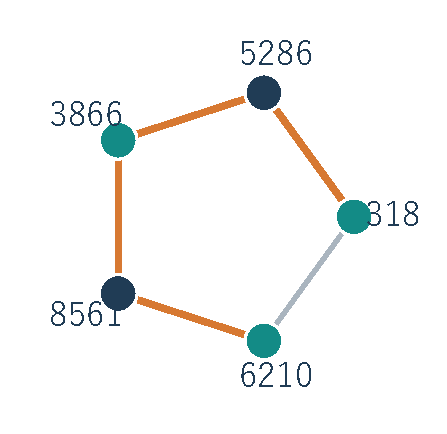
\includegraphics[width=\linewidth,height=48mm,keepaspectratio]{g70_odd_cycle.pdf}
\end{minipage}\hfill\begin{minipage}{.53\textwidth}
\sffamily\bfseries\color{navy}G70の中にも、5頂点の輪がある\par
\normalfont\color{black}\small
318 → 5286 → 3866 → 8561 → 6210 → 318。入力の5辺がすべて存在することを確認した。G70は三角形を持たないが、これだけで二部グラフではないと分かる。
\end{minipage}
\figcap{12}{G70の入力から確認した閉路。数字は入力ファイルの頂点番号。色は図11と同じで、割当ては説明用。実際のCIM出力を描いた図ではない。}
\begin{point}{閉路の「数」だけで未cut数を足してはいけない}
二つの奇数閉路が辺を共有すると、その1本を未cutにすることで両方の条件を満たす場合がある。\textbf{閉路の重なり方}が重要であり、奇数閉路を数えて1本ずつ損失を加算することはできない。
\end{point}
この構造は、複数の辺を同時に満たせない競合を表す。CIMの解析では、単に次数が高い・低いという話から、どの競合する部分で同じ配置へ偏るのかへ視点を進められる。偏りの原因だという結論は、まだ実験で確かめる必要がある。

\newpage
\pagehead{09 / 固有値を一から読む}{固有値は「繰り返しても形が保たれる倍率」}{まず4点の輪で、隣の値を足す操作を考える。}
\sub{隣接行列は、隣の値を集める表}
辺があれば$A_{ij}=1$、なければ0とする。頂点上の数値を並べたベクトル$x$に$A$を掛けると、$(Ax)_i=\sum_{j:\{i,j\}\in E}x_j$となり、各頂点に隣の値の合計が集まる。
\[
A=\begin{pmatrix}0&1&0&1\\1&0&1&0\\0&1&0&1\\1&0&1&0\end{pmatrix},\qquad
x=\begin{pmatrix}1\\-1\\1\\-1\end{pmatrix},\qquad
Ax=\begin{pmatrix}-2\\2\\-2\\2\end{pmatrix}=-2x.
\]
\begin{center}
\begin{tikzpicture}
\foreach \n/\x/\y/\txt/\col in {a/0/0/{+1}/teal,b/0/1.7/{-1}/navy,c/1.7/1.7/{+1}/teal,d/1.7/0/{-1}/navy}{\node[circle,fill=\col,text=white,minimum size=10mm,font=\sffamily] (\n) at(\x,\y){\txt};}
\foreach \a/\b in {a/b,b/c,c/d,d/a}{\draw[light,thick](\a)--(\b);}
\node[box,text width=70mm,right=18mm of c,anchor=west] (t) {隣の2点は、自分と逆符号\\隣を足すと「自分の値 × $-2$」\\形は保たれ、全体の符号と大きさが変わる};
\end{tikzpicture}
\end{center}
\figcap{13}{同じ倍率で形が保たれる配置の例。点の数字がベクトル成分で、緑・紺は正負を示す。灰色は接続。$Ax=\lambda x$を満たす$x$が固有ベクトル、倍率$\lambda$が固有値である。}
\sub{Max-Cutとの接点：隣と逆符号の方向}
正重みの辺では、隣と逆符号になるほどcutに有利である。そのような方向は、正の隣接行列$A$の\textbf{負の側の固有値}と関係する。ただし、固有ベクトルの成分は一般に連続値であり、その符号を取るだけで最適解になる保証はない。[3]
\begin{point}{行列を変えると、固有値の意味も変わる}
\textbf{隣接行列$A$}：隣から値を集める。\\
\textbf{正規化隣接行列$S=D^{-1/2}AD^{-1/2}$}：次数の影響を調整して集める。\\
\textbf{正規化ラプラシアン$L=I-S$}：隣とのずれを見る。\\
$D$は次数を対角に並べた行列。孤立点の扱いを避けるため、以下では辺のある連結成分内で考える。
\end{point}
\source{固有値とMax-Cutの接点は[3]。4点の行列計算と図は本資料の説明用。}

\newpage
\pagehead{10 / スペクトルとCIM}{連結性の固有値と、CIMの増幅方向}{同じ「固有値」という言葉でも、測る目的をそろえる。}
\pic{spectral_connectivity.pdf}{43mm}
\figcap{14}{正規化ラプラシアンの第2小固有値の例。緑は頂点、灰色は重み1の辺、橙は追加する接続辺。接続を強めると、この例では値が大きくなる。説明用の重み付きグラフで、G-setの実測スペクトルではない。}
\sub{連結性を見るなら、第2小固有値}
連結グラフの$L$は最小固有値が0で、第2小固有値$\lambda_2(L)>0$となる。非連結なら0が複数あり、$\lambda_2(L)=0$。そのため、G55/G70全体で0が出ても主要部のつながり方を比較したことにはならない。
\sub{二部性を見るなら、正規化隣接行列の下端}
辺のある連結グラフでは、$S$の最小固有値が$-1$になることと二部グラフであることが対応する。例えば四角形は$-1$、三角形は$-1/2$である。小さな二部成分が混ざるだけでも全体の下端が$-1$になるので、主要部を分けて見る。
\sub{CIMでは、結合行列が振幅の方向を増幅する}
本リポジトリのMax-Cut結合は、正の隣接行列$A$に対して$J=-\alpha A$（$\alpha>0$）の符号を使う。[8] 初期の小振幅で飽和を無視した説明モデルを
\[
c_{t+1}\simeq g(t)(aI+bJ)c_t+\text{雑音}
\]
と書く。$Jv_k=\mu_kv_k$、$c_t=\sum_k z_k(t)v_k$と分解すると、各方向は
\[
z_k(t+1)\simeq g(t)(a+b\mu_k)z_k(t)+\text{雑音の成分}
\]
で増減する。倍率の違いが積み重なれば、ある方向が相対的に強くなる。$A$の最小固有値は、$J=-\alpha A$では最大固有値に対応する。
\begin{caution}{説明モデルと、実際のCIMを分ける}
上式は増幅の意味を示す線形近似であり、完全な更新式ではない。飽和、雑音、ポンプ変化も効く。既存解析でG55/G70の主要固有方向への偏りは観測されたが、構造や固有値だけでG22との差を説明し切ったわけではない。[8]
\end{caution}

\newpage
\pagehead{11 / 最優先の構造評価論文}{MQLib：構造から探索法の得意・不得意を読む}{Dunning・Gupta・Silberholz（2018）[1]を詳しく見る。}
\sub{何をした研究か}
37のMax-Cut/QUBOヒューリスティックを対象に、58の問題特徴量から探索法を選ぶ。各探索法について、5回の試行の平均が比較対象中で最良になるかを予測するランダムフォレストを作り、新しい問題では予測値の高い探索法を選ぶ。[1, Section 6]
\begin{center}\begin{tikzpicture}
\node[box,text width=32mm] (a){グラフ1個\\58種類の特徴量};
\node[box,text width=42mm,right=8mm of a](b){探索法ごとの予測器\\37手法の成績を学習};
\node[box,text width=32mm,right=8mm of b](c){有望な探索法を選ぶ\\選んだ手法で解く};
\draw[flow](a)--(b);\draw[flow](b)--(c);
\end{tikzpicture}\end{center}
\figcap{15}{論文の処理を説明用に整理した図。入力はグラフの特徴であり、同じグラフ上の個別のCIM解を順位付けする図ではない。}
\sub{何が分かったか}
評価対象の2,635問題を学習1,844・評価791に分けた実験では、1手法を選ぶ構成の平均期待偏差は0.08\%、比較に用いたBUR02固定では0.27\%だった。ここでの基準は論文内の最良既知値であり、すべての厳密最適値ではない。[1]
\pic{mqlib_result.pdf}{38mm}
\figcap{16}{論文Section 6の報告値を再描画。灰は固定した探索法、緑は問題特徴から選択した探索法。小さいほど基準の最良既知値に近い。本研究で再実験した結果ではない。}
\sub{今回、取り入れるべき考え方}
この研究が示すのは、\textbf{「普遍的な難しさ」を一つの数で決めるより、構造と探索法の相性を見る}という方針である。今回も「G22は簡単か」だけでなく、「どのCIM条件で、どの構造に対して、どのような出力になるか」と問い直せる。
\begin{point}{まず読む場所と、CIMへの読み替え}
\textbf{Section 2.2}：問題の特徴量をどう選ぶか。\\
\textbf{Section 6}：特徴量から探索法を選び、別の問題で検証する流れ。\\
この枠組みをCIMの構造診断へ使うことは本資料の提案である。候補解の将来価値の評価まで、MQLibが証明したわけではない。
\end{point}
\source{今回は著者公開PDFのSection 2.2・6を確認した。旧版の「本文未精読」から確認範囲を更新。特徴量の詳細は公開CSVと付録を併せて参照する。[1]}

\newpage
\pagehead{12 / ECO-DQNの仕組み}{ECO-DQN：次に反転する点を学ぶ}{Barrettほか（AAAI 2020）[7]。候補を採点するだけのモデルではない。}
\sub{状態・行動・学習する値}
現在の割当てから1頂点を選んで反転する操作を繰り返す。同じ頂点を後で再び反転できるため、一度の判断をやり直せる。MPNNは辺を通じて頂点間の情報を集め、各反転の将来報酬を表すQ値を出力する。[7]
\begin{center}\begin{tikzpicture}
\node[box,text width=32mm](a){グラフ＋現在の割当て\\探索の履歴};
\node[box,text width=35mm,right=8mm of a](b){MPNN\\各頂点のQ値を計算};
\node[box,text width=32mm,right=8mm of b](c){1頂点を反転\\状態と履歴を更新};
\draw[flow](a)--(b);\draw[flow](b)--(c);
\draw[flow](c.south)--++(0,-.6)-|(a.south);
\end{tikzpicture}\end{center}
\figcap{17}{ECO-DQNの探索を説明用に整理した図。各ステップで状態が変わり、Q値も再計算される。グラフだけから一度だけ評価値を出す処理とは異なる。}
\sub{モデルが見る7種類の情報}
\noindent\begin{tabularx}{\textwidth}{@{}p{28mm}X@{}}
\toprule\textbf{範囲} & \textbf{観測する情報}\\\midrule
頂点ごと & ①現在の割当て、②反転直後のcut変化、③最後に反転してからの手数。\\
状態全体 & ④現在のcutと過去最良cutとの差、⑤現在解と過去最良解の距離、⑥直ちに改善する反転の数、⑦残り手数。\\\bottomrule
\end{tabularx}
\sub{報酬が、目先の改善だけに限定されていない}
主な報酬は、それまでの最良cutを更新した分を頂点数で割ったもの。cutを一時的に下げても直接罰せず、初めて到達する局所最適状態への小さな補助報酬も用いる。将来報酬の割引率は0.95である。[7]
\begin{point}{反転直後のgainと、Q値の違い}
反転直後の変化は計算できる。全辺重み1なら
\[
\Delta_i C=\text{頂点$i$につながる未cut辺数}-\text{cut辺数}.
\]
例えば未cutが3本、cutが1本なら、反転直後は2点改善する。これに対してQ値は、\textbf{その反転の後にも探索を続けたときの報酬}を予測する量である。この3対1の例は説明用で、論文の実験値ではない。
\end{point}
\source{方法と7観測は[7]本文のObservations・Rewards。図17とgainの数え方は本資料の説明。Q値はGA/SAの到達品質そのものではない。}

\newpage
\pagehead{13 / ECO-DQNの結果とCIMとの関係}{使えそうな点と、越えてはいけない解釈}{CIMを置き換える話へ進む前に、診断の道具として読む。}
\sub{論文で確かめられた範囲}
200頂点のERグラフで学習したモデルをG-setへ適用した報告では、Table 1の「G22--32」群の平均比率はECO-DQNが0.971、S2V-DQNが0.919だった。この群は各グラフ1エピソードでの評価であり、\textbf{G22単独の値でも、最適解への成功確率でもない}。[7]

著者の補足資料にはSimCIMとの比較もある。ただし、これはCIMが作った解をECO-DQNへ渡す結合実験ではない。SimCIMと本リポジトリの進行波CIMも同一実装ではない。[7]
\sub{CIM研究から離れずに使うなら}
まず学習モデルを導入せず、論文が観測に使う\textbf{反転gain、改善可能な頂点数、過去最良からの距離}を、保存したCIM出力や時間軌跡の診断へ使う。どの局所構造で改善可能性が残り、どの構造で配置が固定されるかを見るためである。これは本資料からの応用案で、実証済みの結果ではない。
\begin{center}\begin{tikzpicture}
\node[box,text width=35mm](a){\textbf{主役：CIM}\\候補と時間軌跡を生成};
\node[box,text width=40mm,right=8mm of a](b){\textbf{まずは診断}\\gain・配置・構造を照合};
\node[box,text width=31mm,right=8mm of b](c){\textbf{説明を深める}\\CIM条件の違いを読む};
\draw[flow](a)--(b);\draw[flow](b)--(c);
\end{tikzpicture}\end{center}
\figcap{18}{今回優先する使い方。CIMで解を生成する部分を維持し、先行研究の観測量を診断へ取り入れる。学習器による後処理を先に主題としない。}
\sub{適用するときの主な懸念}
\noindent\begin{tabularx}{\textwidth}{@{}p{34mm}X@{}}
\toprule\textbf{論点} & \textbf{今回確認が必要なこと}\\\midrule
何の価値か & Q値はECO-DQNの報酬と方策に依存する。GA/SAに渡したときの価値とは異なる。\\
履歴がない初期解 & CIM出力だけでは「最後の反転からの手数」などが決まらない。ゼロに設定するなどの初期化自体が設計選択になる。\\
対象の違い & 学習用の重み・グラフ分布と、正重みのG55/G70の違いを確認する。10,000頂点での性能は未確認。\\
計算費用 & 反転のたびに推論する方法は、大量のCIM候補を一度だけ採点する方法より重くなり得る。\\\bottomrule
\end{tabularx}
\begin{caution}{研究の主語をそろえる}
ECO-DQNの高速化や性能向上そのものを主題にすると、別の学習型探索研究になる。ここでは\textbf{CIMが作る配置を理解するために、何を観測するか}を学ぶのが自然である。
\end{caution}

\newpage
\pagehead{14 / 当面の範囲}{構造とCIMの理解を先に進める}{将来価値の学習と候補選別の詳細設計は、後の課題として残す。}
\sub{いま取り組む問い}
\begin{enumerate}
\item \textbf{どこで得点を失っているか。} 橋・木状部分と主要ブロックを分けて、CIM解のcutを集計する。構造上は簡単な部分でも、現行の探索が満たしているかは別に確かめる。
\item \textbf{どこに共通の配置があるか。} 孤立点の違いと、主要ブロック内の辺のcut状態の違いを区別する。頂点のハミング距離だけでは見えない共通性を調べる。
\item \textbf{どの方向へ増幅されるか。} CIMの結合行列$J$に対する固有方向と、振幅・符号配置の対応を読む。正規化隣接行列やラプラシアンの指標と混同しない。
\end{enumerate}
\begin{point}{仮説を一つの説明に固定しない}
「橋が多いから停滞する」「高次数だから簡単」「主要固有方向だけで決まる」とは、現時点では言えない。グラフの構造、CIM条件、実際の配置を対応させ、\textbf{どの観測ならその説明を支持・否定できるか}を考える段階である。
\end{point}
\sub{Transformerの関心は、構造の表現方法として残す}
GraphGPS [5]は、位置・構造情報、近隣との情報交換、global attentionを組み合わせる。MARCO [6]はGraph TransformerをMax-Cutの探索方策に使う。どちらも参考になるが、今回は「学習器で種を選ぶ」設計を詳しく進めるより、\textbf{どの構造や配置を表現したいのか}を明確にすることを優先する。

将来モデルを比較する場合も、手で計算できる特徴量やMPNNを基準に置く。Transformerを使うこと自体を目的にはせず、構造のどの情報が追加で得られるかを見る。
\sub{後で戻る課題は、一つだけ明記する}
構造とCIM出力の関係が整理できたら、「その情報がGA/SAの初期解としての良さを予測するか」を次の段階で検証する。旧版の詳細な価値関数、教師データ作成、候補選別フローは今回の本文から外した。
\sub{残した先行研究の役割}
\noindent\begin{tabularx}{\textwidth}{@{}p{35mm}X@{}}
\toprule\textbf{論文} & \textbf{ここで読む目的}\\\midrule
MQLib [1] & 構造と探索法の相性を調べる考え方を学ぶ。\\
Rehfeldtほか [2] & 分解できる構造の数学的な意味を押さえる。\\
Trevisan [3] & Max-Cutとスペクトルの接点を押さえる。\\
ECO-DQN [7] & 配置と探索の状態を、どの情報で観測するかを学ぶ。\\\bottomrule
\end{tabularx}

\newpage
\pagehead{15 / 文献と再現情報}{出典と、今回確認した内容}{文献は方法・結果・適用範囲を区別して参照した。}
{\small
\noindent\textbf{[1] Dunning, I.; Gupta, S.; Silberholz, J. (2018).}\\
\textit{What Works Best When? A Systematic Evaluation of Heuristics for Max-Cut and QUBO.} INFORMS Journal on Computing, 30(3), 608--624.\\
\href{https://github.com/MQLib/MQLib/blob/master/paper/SECM_final.pdf}{著者公開本文} / \href{https://github.com/MQLib/MQLib}{公式実装}。Section 2.2・6を確認。

\noindent\textbf{[2] Rehfeldt, D.; Koch, T.; Shinano, Y. (2023).}\\
\textit{Faster exact solution of sparse MaxCut and QUBO problems.} Mathematical Programming Computation, 15, 445--470.\\
\href{https://link.springer.com/article/10.1007/s12532-023-00236-6}{公開全文: DOI 10.1007/s12532-023-00236-6}。Section 4.1の分解を確認。

\noindent\textbf{[3] Trevisan, L. (2009; preprint 2008).}\\
\textit{Max Cut and the Smallest Eigenvalue.} STOC 2009.\\
\href{https://arxiv.org/abs/0806.1978}{著者プレプリント: arXiv:0806.1978}。非負重みMax-Cutのスペクトル法。

\noindent\textbf{[4] Schwartzman, G. (2024).}\\
\textit{Local Max-Cut on Sparse Graphs.} ESA 2024, LIPIcs 308, Article 98.\\
\href{https://drops.dagstuhl.de/entities/document/10.4230/LIPIcs.ESA.2024.98}{論文・PDF}。局所的な疎さとFLIPの平滑化計算量。GA/SAの品質保証ではない。

\noindent\textbf{[5] Rampášek, L. et al. (2022).}\\
\textit{Recipe for a General, Powerful, Scalable Graph Transformer.} NeurIPS 2022.\\
\href{https://arxiv.org/abs/2205.12454}{論文: arXiv:2205.12454}。効率的attentionを選ぶ構成と、通常の全点attentionを区別する。

\noindent\textbf{[6] Garmendia, A. I.; Cappart, Q.; Ceberio, J.; Mendiburu, A. (2024).}\\
\textit{MARCO: A Memory-Augmented Reinforcement Framework for Combinatorial Optimization.} IJCAI 2024, 6931--6939.\\
\href{https://www.ijcai.org/proceedings/2024/0766.pdf}{公開本文PDF}。Section 5のGraph Transformerを参照。

\noindent\textbf{[7] Barrett, T. D.; Clements, W. R.; Foerster, J. N.; Lvovsky, A. I. (2020).}\\
\textit{Exploratory Combinatorial Optimization with Reinforcement Learning.} AAAI, 34(04), 3243--3250.\\
\href{https://ojs.aaai.org/index.php/AAAI/article/view/5723}{出版版} / \href{https://arxiv.org/abs/1909.04063}{本文・補足資料} / \href{https://github.com/tomdbar/eco-dqn}{公式実装}。観測・報酬・Table 1・SimCIM比較を確認。

\noindent\textbf{[8] 本リポジトリの記録・実装。}\\
\texttt{modules/CIM.py}、2026年8月23日のCIMアブレーション、9月14日のGA世代別多様性測定。図10の値は後者の\texttt{REPORT.md}に基づく。確認した実験結果は9月14日分まで。
}
\sub{追加図と集計の再現}
{\small
同梱の\texttt{data/summary.json}に既存の構造集計、\texttt{degree\_and\_cycle.json}に今回の次数分布とG70の閉路、\texttt{toy\_spectrum.json}に小グラフの固有値を保存した。図8は既存の構造集計、図9は新たな次数集計、図10は既存GA結果の正規化、図12は入力で確認した閉路、図16は文献の報告値であり、説明用の例と区別した。

\texttt{make\_revision\_figures.py}が追加図を生成する。入力の構造集計は、リポジトリの\texttt{graph\_structure\_audit.py}で再実行できる。赤字ごとの反映先は\texttt{redline\_response.md}に記録した。元PDFと旧版は保持している。
}
\end{document}
